% Written by Francois Fleuret <francois@fleuret.org>
% https://twitter.com/francoisfleuret/status/1529744066086424577.

% Original TikZ source: https://fleuret.org/git-extract/tex/single-attention.tex

% Any copyright is dedicated to the Public Domain.
% https://creativecommons.org/publicdomain/zero/1.0

\documentclass[tikz]{standalone}

\usepackage{mathtools}
\def\transpose{^{\top}}
\DeclareMathOperator\softmax{softmax}
\DeclareMathOperator\Attention{Attention}

\usetikzlibrary{positioning, arrows.meta}

\begin{document}

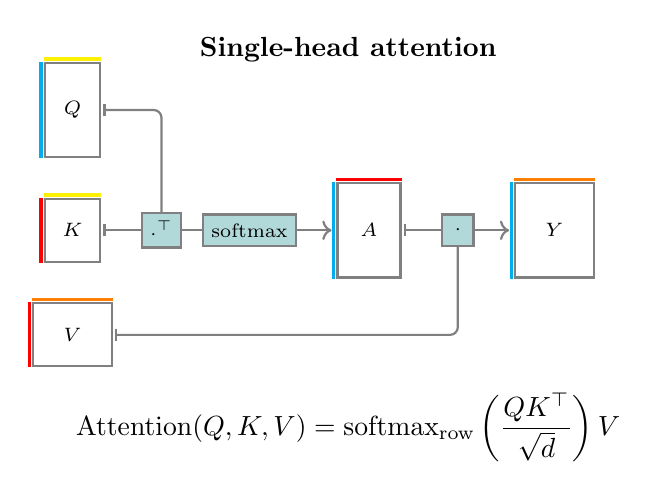
\begin{tikzpicture}[
  value/.style = {
    font=\scriptsize, rectangle, draw=black!50, fill=white,   thick,
    inner sep=3pt, inner xsep=2pt, minimum size=10pt, minimum height=20pt
  },
  parameter/.style = {
    font=\scriptsize, rectangle, draw=black!50, fill=lightblue!15, thick,
    inner sep=0pt, inner xsep=2pt, minimum size=10pt, minimum height=20pt
  },
  operation/.style = {
    font=\scriptsize, rectangle,    draw=black!50, fill=teal!30, thick,
    inner sep=3pt, minimum size=10pt, minimum height=20pt
  },
  flow/.style={->,shorten <= 1pt,shorten >= 1pt, draw=black!50, thick},
  f2f/.style={draw=black!50, thick},
  v2f/.style={{Bar[width=1.5mm]}-,shorten <= 0.75pt,draw=black!50, thick},
  f2v/.style={->,shorten >= 0.75pt,draw=black!50, thick}
]

  \node[font=\bfseries] at (3.5, 2.3) {Single-head attention};
  \node at (3.5, -2.5) {$\displaystyle \Attention(Q, K, V) = \softmax_\text{row} \left( \frac{Q K\transpose}{\sqrt{d}} \right) V$};
  \node[value,    minimum height=0.8cm,minimum width=0.7cm] (K) at (0, 0) {$K$};
  \node[value,    minimum height=1.2cm,minimum width=0.7cm] (Q) [above=0.5cm of K] {$Q$};
  \node[value,    minimum height=0.8cm,minimum width=1.0cm] (V) [below=0.5cm of K] {$V$};
  \node[operation,minimum height=0.4cm,minimum width=0.4cm] (att) [right=0.5cm of K] {$\cdot\transpose$};
  \node[operation,minimum height=0.4cm,minimum width=0.4cm] (sm) [right=0.25cm of att] {$\softmax$};
  \node[value,    minimum height=1.2cm,minimum width=0.8cm] (A) [right=0.5cm of sm] {$A$};
  \node[operation,minimum height=0.4cm,minimum width=0.4cm] (prod) [right=0.5cm of A] {$\cdot$};
  \node[value,    minimum height=1.2cm,minimum width=1.0cm] (Y) [right=0.5cm of prod] {$Y$};

  \draw[v2f,rounded corners=1mm] (K) -- (att);
  \draw[v2f,rounded corners=1mm] (Q) -| (att);
  \draw[f2f,rounded corners=1mm] (att) -- (sm);
  \draw[f2v,rounded corners=1mm] (sm) -- ([xshift=-1pt]A.west);

  \draw[v2f,rounded corners=1mm] (A) -- (prod);
  \draw[v2f,rounded corners=1mm] (V) -| (prod);
  \draw[f2v,rounded corners=1mm] (prod) -- ([xshift=-1pt]Y.west);

  \draw[very thick,yellow] ([yshift=1pt]Q.north west) -- ([yshift=1pt]Q.north east);
  \draw[very thick,yellow] ([yshift=1pt]K.north west) -- ([yshift=1pt]K.north east);
  \draw[very thick,orange] ([yshift=1pt]V.north west) -- ([yshift=1pt]V.north east);
  \draw[very thick,orange] ([yshift=1pt]Y.north west) -- ([yshift=1pt]Y.north east);

  \draw[very thick,red] ([xshift=-1pt]V.north west) -- ([xshift=-1pt]V.south west);
  \draw[very thick,red] ([xshift=-1pt]K.north west) -- ([xshift=-1pt]K.south west);
  \draw[very thick,cyan] ([xshift=-1pt]Q.north west) -- ([xshift=-1pt]Q.south west);
  \draw[very thick,cyan] ([xshift=-1pt]Y.north west) -- ([xshift=-1pt]Y.south west);

  \draw[very thick,cyan] ([xshift=-1pt]A.north west) -- ([xshift=-1pt]A.south west);
  \draw[very thick,red] ([yshift=1pt]A.north west) -- ([yshift=1pt]A.north east);

\end{tikzpicture}

\end{document}
